\documentclass[
	letterpaper, % Paper size, specify a4paper (A4) or letterpaper (US letter)
	10pt, % Default font size, specify 10pt, 11pt or 12pt
]{CSUniSchoolLabReport}


\usepackage{fancyvrb}
\usepackage{multicol}
\usepackage{subcaption}

\captionsetup[subfigure]{labelformat=empty}

\title{Estimating the elementary charge with the Millikan experiment.}

\author{Sebastien \textsc{Psarianos}\\ Sofiya \textsc{P'yavka}}

\date{\today}

\begin{document}

\maketitle

\section{Introduction}
The objective of this experiment was to determine the elementary charge using a Millikan apparatus.
Oil droplets are electrically charged due to the friction they experience in the capillary of the
apparatus' atomizer and then enter a chamber that consists of two charged  parallel plates which
produce a constant electric field. Three forces then act on the oil droplets; the downward gravitational
force $F_g = m_og$ where $m_o$ is the mass of the oil droplet and $g$ is the gravitational acceleration,
the upward buoyant force $F_g=-m_ag$ where $m_a$ is the mass of the air displaced by the oil droplet,
the electric force $F_E=QE$ where $Q$ is the charge of the oil droplet and $E$ is the electric field and
Stokes' resistive force $F_d=6\pi r \eta\nu$ where $r$ is the radius of the spherical oil
droplet, $\eta$ is the viscosity and $\nu$ is the velocity under laminar flow conditions.
Depending on the set voltage, the motion of the oil droplet changes as follows;\\

i) If the oil droplet is floating in the chamber, the net force is zero which can be described by:
$$g(m_o-m_a)-\frac{QV_{stop}}{d}=0$$
\begin{center}
    \textbf{Equation 1: Static particle equation}
\end{center}
Where $V_{stop}$ is the voltage which allows the droplet to remain suspended and $d$ is the
distance between the charged parallel plates.\\

ii) If the droplet is moving downward with terminal velocity $\nu_t$, the net force is zero
and can be described by:
$$g(m_o-m_a)-6\pi r \eta\nu_t=0$$
\begin{center}
    \textbf{Equation 2: Terminal falling velocity equation}
\end{center}

iii) If the oil droplet is accelerating upwards the equation of motion is described by
$$ma=-g(m_o-m_a)+QE- 6\pi r \eta\nu$$
\begin{center}
    \textbf{Equation 3: Upwards accelerating droplet equation}
\end{center}


The elementary charge can then be determined using two methods. If the experimenter determines the
stopping voltage and terminal velocity of an oil droplet, the following equation can be derived from
\textbf{Equation 1} and \textbf{Equation 2}.

$$Q = C \frac{v_t^{\frac{3}{2}}}{v_{stop}}$$
\begin{center}
    \textbf{Equation 4: Method one charge calculation model}
\end{center}

Where $C$ is a constant defined by:

$$C = \frac{18\pi d \eta^\frac{3}{2}}{\sqrt2 \sqrt{\rho_o-\rho_a}\sqrt g}$$
\begin{center}
    \textbf{Constant 1}
\end{center}

Where the densities $\rho_o = \frac{3m_o}{4\pi r^3}$ and $\rho_a = \frac{3m_a}{4\pi r^3}$\\

Furthermore, if the experimenter determines the terminal velocity of the oil drop, the voltage
$V_{up}$ at which the oil droplet is moving upward with a constant speed $\nu_2$, the following
equation can be derived from \textbf{Equations 1,2 and 3};

$$Q = C(\nu_1 + \nu_2)\frac{\nu_t^\frac{1}{2}}{\nu_{up}}$$
\begin{center}
    \textbf{Equation 5: Method two charge calculation model}
\end{center}
Where the constant $C$ is the same one determined using the first method. Using
either method, the greatest common divisor of the individual experimental oil
droplet charges can be found, which should then correspond to the value of the
elementary charge as the experimental charges should be integer multiples of
the elementary charge.
\newpage
\section{Methodology and Procedure}
This experiment was a replication of the Millikan oil drop experiment. The experimental apparatus
consisted of a variable voltage power supply connected to two plates making up the top and bottom
of a transparent observation chamber. A Hewlett-Packard 3476A Digital Multimeter set to a range of 1100 V was connected
to the terminals on the chamber to measure the
voltage across the plates. This created an approximately uniform electric field within the
chamber. An atomizer was connected to the chamber that allowed for charged oil droplets to be sprayed
into the chamber. A camera that was attached to a microscopic lens was set up to point inside chamber and
provided the ability to track individual droplets' vertical position using a computer program. This experimental
apparatus is shown in \textbf{Figure 1}.\\

\begin{figure}[H]
	\centering
	\begin{subfigure}{0.45\textwidth}
		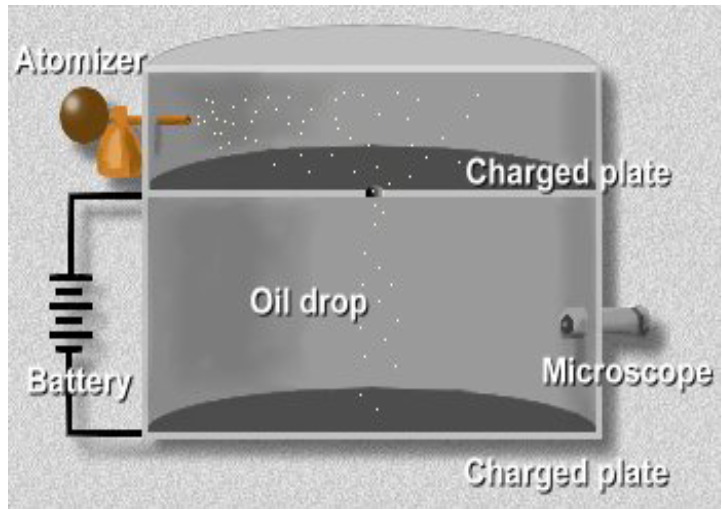
\includegraphics[width=\textwidth]{../figures/apparatusDiagram.png}
		\caption{\textbf{Figure 1: Experimental apparatus diagram}}
	\end{subfigure}
\end{figure}
For each measurement, the following procedure was followed. The power supply was set to a value that was approximately
in the middle of its output range (generally $\sim 300V$). The atomizer was used to spray a mist of droplets into
the chamber.
% What makes a good droplet?
Once an appropriate droplet was located, the camera was moved and focused to get an ideal image for tracking, allowing
the computer program to track the droplet's vertical position. The voltage was then adjusted until the droplet was stationary,
and the value was recorded as the stopping voltage and the computer program was set up to track the vertical position of the
droplet.\\

Adjusting the voltage on the power supply to $0V$ eliminated the electric field within the chamber.
The droplet was allowed to accelerate and then, once it had reached a constant velocity, the position
values were saved to a spreadsheet for a small interval of time. These position values in units of pixels
were used to calculate
the terminal velocity of the droplet.\\

The power supply was then returned to the previously determined stopping voltage to
stop the movement. The power supply was then increased to a value larger than the stopping voltage. This voltage
value was recorded with the corresponding stopping voltage. The same tracking technique was used to get
a set of positions as the particle traveled upwards and used to calculate the upwards velocity.\\

\section{Results}
Note, all referenced functions, equations and constants can be found in the appendix.\\

To determine the uncertainty of the stopping and upward voltages, \textbf{Function 1}
was defined based off of the Hewlett-Packard 3476A Digital Multimeter specifications.\\

To find the charge of the oil droplet for each trial, the terminal velocity and constant
upward velocity had to be determined from the experimental data. To convert the
position data from pixels to units of meters, the position data was divided by
a factor of 540000 since the calibration factor of the left camera was found to
be $(540 \pm 1) px/mm$. Since the camera had a frame rate of $10 Hz$, for each individual
trial and its respective position data set, an array of times was generated where the
time elapsed per frame was $0.1 s$. The two sets of position and time data were then
fitted to a linear model as implemented by \textbf{Function 2} by passing them through \lstinline{scipy}'s
\lstinline{curve_fit} function. The uncertainty was determined using \lstinline{curve_fit}'s
covariance values since the diagonals of the covariance matrix represent the variability
of each parameter and the square root of this was taken to calculate the standard error.
From this an array of terminal and constant upward velocities was determined.\\

Note \textbf{Constant 1} was derived using \textbf{Equation 1}, \textbf{Equation 2} and \textbf{Equation 3} and its
numerical value, $2.0\times10^{-10}\frac{kg}{s^{1/2}m^{1/2}}$ was determined using known physical constants which can be found in the appendix.\\

{\large\textbf{Method 1}}\\

\textbf{Equation 4} as implemented by \textbf{Function 3} was used to generate an array of charges for
each individual trial by passing in the stopping voltage and terminal velocity arrays. The uncertainties
of the charges was determined using \textbf{Equation 6} as implemented by \textbf{Function 5}.\\

{\large\textbf{Method 2}}\\

\textbf{Equation 5} as implemented by \textbf{Function 4} was used to generate an array of charges for
each individual trial by passing in the terminal velocity, constant upward velocity and upward voltage
arrays. The uncertainties of the charges was determined using \textbf{Equation 7} as implemented by
\textbf{Function 6}.\\

Histograms for both methods were then generated as depicted in \textbf{Figure 2} and \textbf{Figure 3}.
\textbf{Function 7} was used to determine the average uncertainty of the charges for both methods.\\

\begin{figure}[H]
	\begin{subfigure}{0.45\textwidth}
		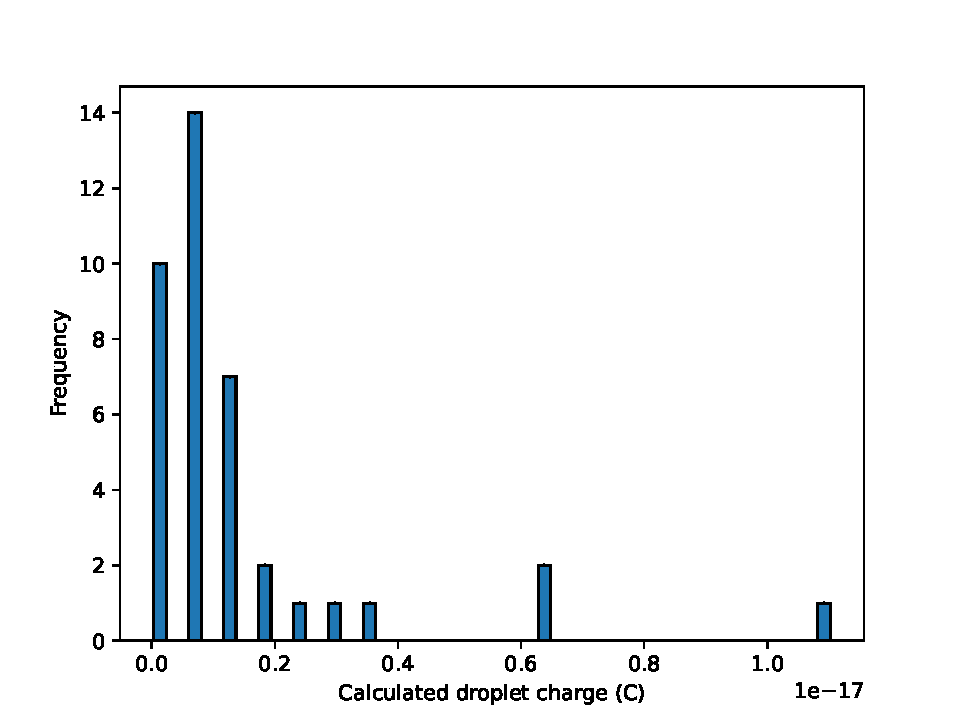
\includegraphics[width=\textwidth]{../figures/methodOneHistogram.pdf}
		\caption{\textbf{Figure 2: Histogram showing the frequency of droplet charges as calculated with method one}}
	\end{subfigure}\hfill
	\begin{subfigure}{0.45\textwidth}
		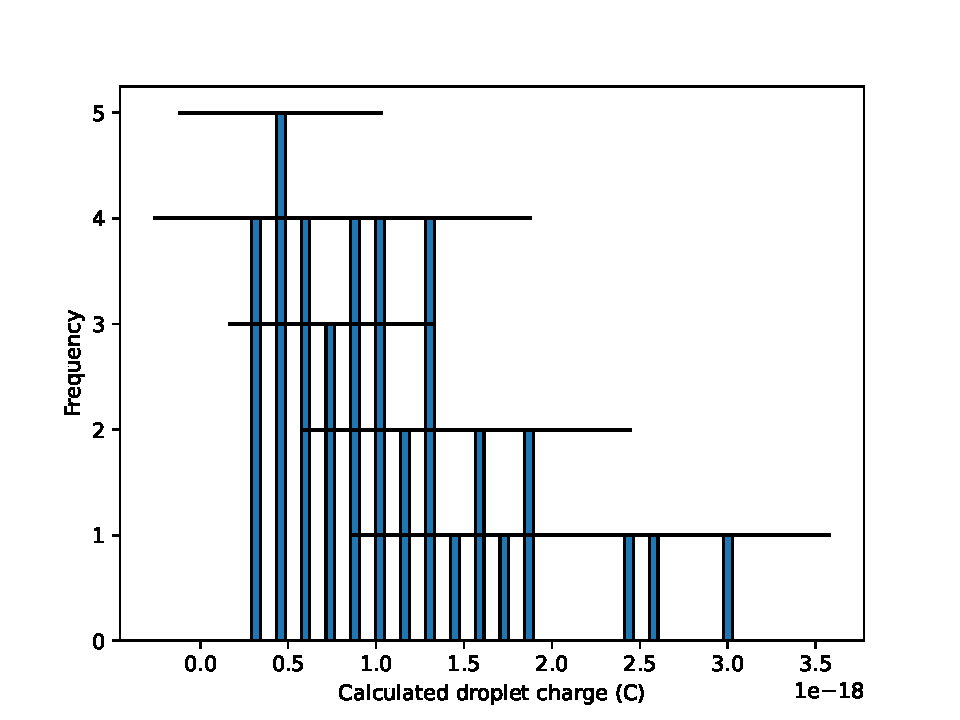
\includegraphics[width=\textwidth]{../figures/methodTwoHistogram.pdf}
		\caption{\textbf{Figure 3: Histogram showing the frequency of droplet charges as calculated with method two}}
	\end{subfigure}
\end{figure}


The values that had been determined with \textbf{Functions 4, 5, 6 and 7} were all not in line with the measurement precision
which required 3 significant figures. Additionally, a requirement of greatest common divisor calculation in \lstinline{numpy} is that the
values must all be of the \lstinline{int} type. \textbf{Function 8} was defined to resolve both of these issues.
The function is supplied with a list and the required number of significant figures. The function will then return a list that
represents the values rounded to three significant figures and scaled up to integers, as well as the scaling factor that
the values were scaled by. For example $1.234\times10^{-19}$ and $5.678\times 10^{-20}$ will be scaled to $1230$ and $568$
respectively and the scaling factor will be $20$. \\

This function was applied both to the results for method one and method two and additionally was applied to the uncertainty of each
measurement for the purpose of error propagation. This satisfied the requirements of the values being integers and ensured that
the values had the correct precision. The \lstinline{numpy} \lstinline{gcd} function was then used to calculate the greatest common
divisor of all four data sets and then the values were returned to their original order of magnitude by dividing by ten to the power
of the scaling factor returned from \textbf{Function 8}.\\


To determine the average radius of an oil droplet, the average terminal velocity was determined using \lstinline{numpy}'s
\lstinline{average} function and \textbf{Equation 8}.
\newpage


\section{Analysis and Discussion}
The value of the elementary charge determined using methods 1 and 2 were
$1.0\times 10^{-21}\pm 1.0\times 10^{-23}C$ and $1.0\times 10^{-21}\pm 1.0\times 10-21C$
respectively, however the accepted value of $1.6\times 10^{-19}$ does not fall within the range of uncertainty for
either measurement. To determine the uncertainties of the experimental elementary charges, the greatest common
divisors of the individual charge uncertainties were determined, as they similarly would have been scalar multiples
of their respective experimental elementary charge's uncertainty. Obtaining experimental charge values that are perfect
integer multiples of the accepted value is difficult as measurements such as the voltage can fluctuate during data
collection. Furthermore, rounding may have also been a source of error. When the gcd function was applied to the output of
\textbf{Function 8}, none of the data sets had a common factor greater than one. This meant that when the calculated value
was scaled down to the appropriate order of magnitude, the value was just one divided by the scaling factor from \textbf{Function 8}.
It follows that using the method of determining the greatest common divisor did not yield accurate results.\\

Despite the inaccuracy of the determined values, examining \textbf{Figure 2} and \textbf{Figure 3}, the smallest experimental
charge values of the droplets fell within the same order of the accepted elementary charge value, $10^{-19}$. Furthermore, almost
all charge values for both methods, except one which can be considered as an outlier, were greater than the accepted value of
the elementary charge. Using method 1, the minimum value found disregarding the outlier was $2.6\times10^{-19}\pm 1.6\times10^{-19}C$.
Using method 2, the minimum value found was $3.2\times10^{-19}\pm8.7\times10^{-19}C$. The accepted value falls within the range
of uncertainty for both values and so the minimum experimental droplet charges ultimately act as better estimates of the true
elementary charge value.\\

The average droplet radius found was $1.1\times 10^{-6}m$. Droplets with larger radii were easier to track using the
tracking software since droplets with smaller radii would often dissipate during data collection and the trial would have to
be redone. In regards to the buoyant force, the mass of the displaced air can be determined by $m_a=\frac 43r^3\rho_a$.
Furthermore, the mass of the oil droplet can be determined by $m_o=\frac 43r^3\rho_o$ and since $\rho_o >> \rho_a$, it follows that
$m_o>>m_a$. In \textbf{Equation 1}, \textbf{Equation 2} and \textbf{Equation 3}, the difference between the masses only matters.
Thus, the buoyant force is not significant in this experiment.
\section{Conclusion}
Although the experimental elementary charges using both methods and finding their greatest common divisors did not yield accurate
values, examining \textbf{Figure 2} and \textbf{Figure 3} confirms that the charge of the droplets cannot fall below the accepted value. It
follows that the elementary charge can be quantified using the Millikan apparatus and corresponding equations, however,
it is difficult to do so as various sources of error as discussed in the previous section may heavily skew the experimental
results.

\newpage
\section{Appendix}
{\Large\textbf{Constants}}\\
\begin{tabular}{p{0.45\linewidth} p{0.45\linewidth}}
    $$C = \frac{18\pi d \eta^\frac{3}{2}}{\sqrt2 \sqrt{\rho_o-\rho_a}\sqrt g}$$
    \begin{center}
        \textbf{Constant 1}
    \end{center}
\end{tabular}\\

{\Large\textbf{Equations}}\\

\begin{tabular}{p{0.45\linewidth} p{0.45\linewidth}}
    $$g(m_o-m_a)-\frac{Qv_{stop}}{d}=0$$
    \begin{center}
        \textbf{Equation 1: Static particle equation}
    \end{center}
    &
    $$g(m_o-m_a)-6\pi r \eta\nu_t=0$$
    \begin{center}
        \textbf{Equation 2: Terminal falling velocity equation}
    \end{center}
    \\
    $$ma=-g(m_o-m_a)+QE- 6\pi r \eta\nu$$
    \begin{center}
        \textbf{Equation 3: Upwards accelerating droplet equation}
    \end{center}
    &
    $$Q = C \frac{v_t^{\frac{3}{2}}}{V_{stop}}$$
    \begin{center}
        \textbf{Equation 4: Method one charge calculation model}
    \end{center}
    \\
    $$Q = C(\nu_1 + \nu_2)\frac{\nu_t^\frac{1}{2}}{\nu_{up}}$$
    \begin{center}
        \textbf{Equation 5: Method two charge calculation model}
    \end{center}
    &
    $$u(Q(x,y)) = \sqrt{\left(\frac{3c}{2}\frac{x^\frac{1}{2}}{y}\right)^2(u(x))^2 + \left(\frac{-Cx^\frac{3}{2}}{y^2}\right)(u(y))^2}$$
    \begin{center}
        \textbf{Equation 6: Method one charge calculation error propagation (derived from general uncertainty propagation equation)}
    \end{center}
\end{tabular}\\
\begin{center}
    $$u(Q(x,y,z)) =
    \sqrt{
        \left(
            \frac{3}{2}\frac{C}{z}x^\frac12 + \frac{1}{2}C\frac{y}{zx^\frac12}
        \right)^2(u(x))^2 +
        \left(
            \frac{Cx^\frac{1}{2}}{z}
        \right)^2(u(y))^2 +
        \left(
            \frac{-Cx^\frac{3}{2}}{z^2} - \frac{Cyx^\frac12}{z^2}
        \right) ^2 (u(z))^2
    }
    $$
    \textbf{Equation 7: Method two charge calculation error propagation (derived from general uncertainty propagation equation)}
\end{center}

$$r = \sqrt{\frac{\frac 92 \eta v_t}{g\rho_o-\rho_a}} = \frac{3\sqrt \eta\sqrt{v_t}}{\sqrt 2 \sqrt g \sqrt{\rho_o - \rho_a}}$$
\begin{center}
    \textbf{Equation 8: Equation used to calculate average terminal velocity}
\end{center}
\newpage
{\Large\textbf{Functions}}\\
\begin{verbatim}
    def uncertaintyVoltage(reading, ran):
        return 0.006 * reading + 0.001 * ran
\end{verbatim}
\begin{center}
    \textbf{Function 1: Function used to calculate voltage uncertainty}
\end{center}

\begin{verbatim}
def linear(time, velocity, intercept):
    return time * velocity + intercept
\end{verbatim}
\begin{center}
    \textbf{Function 2: General linear model}
\end{center}

\begin{verbatim}
def chargeMethodOne(velocityOne, voltageOne):
    return constant * velocityOne ** (3 / 2) / voltageOne
\end{verbatim}
\begin{center}
    \textbf{Function 3: Method one charge model (implements Equation 4)}
\end{center}

\begin{verbatim}
    def chargeMethodTwo(velocityOne, velocityTwo, voltageTwo):
    return (
        constant
        * (abs(velocityOne) + velocityTwo)
        * abs(velocityOne) ** (1 / 2)
        / voltageTwo
    )
    \end{verbatim}
\begin{center}
    \textbf{Function 4: Method two charge model (implements Equation 5)}
\end{center}

\begin{verbatim}
    def uncertaintyChargeMethodOne(
        velocityOne, voltageOne, uncertaintyOne, uncertaintyTwo
    ):
        return np.sqrt(
            (3 * constant / 2 * np.sqrt(abs(velocityOne)) / voltageOne) ** 2
            * uncertaintyOne ** 2
            + (-1 * constant * abs(velocityOne) ** (3 / 2) / voltageOne ** 2) ** 2
            * uncertaintyTwo ** 2
        )
    \end{verbatim}
\begin{center}
    \textbf{Function 5: Method one uncertainty propagation (implements Equation 6)}
\end{center}
\newpage
\begin{verbatim}
    def uncertaintyChargeMethodTwo(
        velocityOne,
        velocityTwo,
        voltageTwo,
        uncertaintyOne,
        uncertaintyTwo,
        uncertaintyThree,
    ):
        return np.sqrt(
            (
                (3 * constant / 2 * np.sqrt(abs(velocityOne)))
                + (
                    constant
                    / 2
                    * velocityTwo
                    / voltageTwo
                    / np.sqrt(abs(velocityOne))
                )
            )
            ** 2
            * uncertaintyOne ** 2
            + (constant * np.sqrt(abs(velocityOne)) / voltageTwo) ** 2
            * uncertaintyTwo ** 2
            + (
                (-1 * constant * abs(velocityOne) ** (3 / 2) / voltageTwo ** 2)
                - (
                    constant
                    * velocityTwo
                    * np.sqrt(abs(velocityOne))
                    / voltageTwo ** 2
                )
            )
            ** 2
            * uncertaintyThree ** 2
        )
    \end{verbatim}
\begin{center}
    \textbf{Function 6: Method two uncertainty propagation (implements Equation 7)}
\end{center}

\begin{verbatim}
def averageUncertainty(uncertainty):
    s = 0
    for value in uncertainty:
        s += value ** 2
    return np.sqrt(s) / len(uncertainty)
\end{verbatim}
\begin{center}
    \textbf{Function 7: Function used to calculate average uncertainty for histogram}
\end{center}
\newpage
\begin{verbatim}
def scaleAndRound(data, sigFigs):
    """
    Returns a length two tuple. The first element is the values in <data> scaled
    by the order of magnitude of the smalest element in <data> and rounds them
    to the number of significant figures defined in <sigFigs>. The second
    element is the factor that all of the values are scaled by.
    """
    scaleFactor = -(math.floor(math.log(min(data), 10)) - sigFigs + 1)
    scaled = np.rint((data * 10 ** scaleFactor).astype(float)).astype(int)
    for i in range(len(scaled)):
        nonSigDigits = len(str(scaled[i])) - sigFigs
        if nonSigDigits != 0:
            scaled[i] = round(scaled[i], -nonSigDigits)
    return (scaled, scaleFactor)
\end{verbatim}
\begin{center}
\textbf{Function 8: Function used to prepare data sets for greatest common divisor calculation}
\end{center}
\newpage
{\Large\textbf{Data}}
\begin{figure}[H]
	\centering
	\begin{subfigure}{0.45\textwidth}
        \begin{tabular}{| p{0.2\textwidth} | p{0.6\textwidth} |}
\hline
Sample & Charge as calculated with method one (C)\\
\hline
$1$ & $5.14\times 10^{-19} \pm 6.1\times10^{-21}$\\
$2$ & $3.28\times 10^{-19} \pm 3.49\times10^{-21}$\\
$3$ & $1.02\times 10^{-18} \pm 6.83\times10^{-20}$\\
$4$ & $1.2\times 10^{-18} \pm 1.4\times10^{-20}$\\
$5$ & $1.02\times 10^{-18} \pm 1.6\times10^{-20}$\\
$6$ & $4.27\times 10^{-19} \pm 5.23\times10^{-21}$\\
$7$ & $1.98\times 10^{-18} \pm 2.74\times10^{-20}$\\
$8$ & $2.61\times 10^{-19} \pm 4.61\times10^{-21}$\\
$9$ & $6.73\times 10^{-18} \pm 1.57\times10^{-19}$\\
$10$ & $1.82\times 10^{-18} \pm 2.66\times10^{-20}$\\
$11$ & $8.07\times 10^{-19} \pm 1.89\times10^{-20}$\\
$12$ & $3.58\times 10^{-19} \pm 4.84\times10^{-21}$\\
$13$ & $1.58\times 10^{-18} \pm 1.98\times10^{-20}$\\
$14$ & $1.4\times 10^{-18} \pm 1.48\times10^{-20}$\\
$15$ & $2.36\times 10^{-18} \pm 3.41\times10^{-20}$\\
$16$ & $1.65\times 10^{-18} \pm 1.63\times10^{-20}$\\
$17$ & $1.39\times 10^{-18} \pm 1.38\times10^{-20}$\\
$18$ & $1.15\times 10^{-17} \pm 2.48\times10^{-19}$\\
$19$ & $1.15\times 10^{-18} \pm 1.24\times10^{-20}$\\
$20$ & $4.67\times 10^{-19} \pm 4.27\times10^{-21}$\\
$21$ & $7.33\times 10^{-19} \pm 8.32\times10^{-21}$\\
$22$ & $7.44\times 10^{-19} \pm 8.09\times10^{-21}$\\
$23$ & $3.27\times 10^{-19} \pm 3.16\times10^{-21}$\\
$24$ & $1.03\times 10^{-18} \pm 9.63\times10^{-21}$\\
$25$ & $1.29\times 10^{-18} \pm 1.36\times10^{-20}$\\
$26$ & $1.34\times 10^{-19} \pm 1.53\times10^{-21}$\\
$27$ & $9.53\times 10^{-19} \pm 1.06\times10^{-20}$\\
$28$ & $6.64\times 10^{-18} \pm 9.25\times10^{-20}$\\
$29$ & $1.1\times 10^{-18} \pm 1.34\times10^{-20}$\\
$30$ & $1.03\times 10^{-18} \pm 1.32\times10^{-20}$\\
$31$ & $8.77\times 10^{-19} \pm 8.96\times10^{-21}$\\
$32$ & $5.26\times 10^{-19} \pm 5.73\times10^{-21}$\\
$33$ & $1.44\times 10^{-18} \pm 1.9\times10^{-20}$\\
$34$ & $2.52\times 10^{-18} \pm 2.79\times10^{-20}$\\
$35$ & $3.08\times 10^{-19} \pm 2.86\times10^{-21}$\\
$36$ & $9.01\times 10^{-19} \pm 1.35\times10^{-20}$\\
$37$ & $1.26\times 10^{-18} \pm 1.59\times10^{-20}$\\
$38$ & $3.97\times 10^{-18} \pm 6.05\times10^{-20}$\\
$39$ & $3.32\times 10^{-18} \pm 4.62\times10^{-20}$\\
\hline
\end{tabular}

		\caption{\textbf{Table 1: Calculated charge values for each sample using method one }}
	\end{subfigure}
    \hfill
    \begin{subfigure}{0.45\textwidth}
        \begin{tabular}{| p{0.2\textwidth} | p{0.6\textwidth} |}
\hline
Sample & Charge as calculated with method one (C)\\
\hline
$1$ & $5.14\times 10^{-19} \pm 6.1\times10^{-21}$\\
$2$ & $3.28\times 10^{-19} \pm 3.49\times10^{-21}$\\
$3$ & $1.02\times 10^{-18} \pm 6.83\times10^{-20}$\\
$4$ & $1.2\times 10^{-18} \pm 1.4\times10^{-20}$\\
$5$ & $1.02\times 10^{-18} \pm 1.6\times10^{-20}$\\
$6$ & $4.27\times 10^{-19} \pm 5.23\times10^{-21}$\\
$7$ & $1.98\times 10^{-18} \pm 2.74\times10^{-20}$\\
$8$ & $2.61\times 10^{-19} \pm 4.61\times10^{-21}$\\
$9$ & $6.73\times 10^{-18} \pm 1.57\times10^{-19}$\\
$10$ & $1.82\times 10^{-18} \pm 2.66\times10^{-20}$\\
$11$ & $8.07\times 10^{-19} \pm 1.89\times10^{-20}$\\
$12$ & $3.58\times 10^{-19} \pm 4.84\times10^{-21}$\\
$13$ & $1.58\times 10^{-18} \pm 1.98\times10^{-20}$\\
$14$ & $1.4\times 10^{-18} \pm 1.48\times10^{-20}$\\
$15$ & $2.36\times 10^{-18} \pm 3.41\times10^{-20}$\\
$16$ & $1.65\times 10^{-18} \pm 1.63\times10^{-20}$\\
$17$ & $1.39\times 10^{-18} \pm 1.38\times10^{-20}$\\
$18$ & $1.15\times 10^{-17} \pm 2.48\times10^{-19}$\\
$19$ & $1.15\times 10^{-18} \pm 1.24\times10^{-20}$\\
$20$ & $4.67\times 10^{-19} \pm 4.27\times10^{-21}$\\
$21$ & $7.33\times 10^{-19} \pm 8.32\times10^{-21}$\\
$22$ & $7.44\times 10^{-19} \pm 8.09\times10^{-21}$\\
$23$ & $3.27\times 10^{-19} \pm 3.16\times10^{-21}$\\
$24$ & $1.03\times 10^{-18} \pm 9.63\times10^{-21}$\\
$25$ & $1.29\times 10^{-18} \pm 1.36\times10^{-20}$\\
$26$ & $1.34\times 10^{-19} \pm 1.53\times10^{-21}$\\
$27$ & $9.53\times 10^{-19} \pm 1.06\times10^{-20}$\\
$28$ & $6.64\times 10^{-18} \pm 9.25\times10^{-20}$\\
$29$ & $1.1\times 10^{-18} \pm 1.34\times10^{-20}$\\
$30$ & $1.03\times 10^{-18} \pm 1.32\times10^{-20}$\\
$31$ & $8.77\times 10^{-19} \pm 8.96\times10^{-21}$\\
$32$ & $5.26\times 10^{-19} \pm 5.73\times10^{-21}$\\
$33$ & $1.44\times 10^{-18} \pm 1.9\times10^{-20}$\\
$34$ & $2.52\times 10^{-18} \pm 2.79\times10^{-20}$\\
$35$ & $3.08\times 10^{-19} \pm 2.86\times10^{-21}$\\
$36$ & $9.01\times 10^{-19} \pm 1.35\times10^{-20}$\\
$37$ & $1.26\times 10^{-18} \pm 1.59\times10^{-20}$\\
$38$ & $3.97\times 10^{-18} \pm 6.05\times10^{-20}$\\
$39$ & $3.32\times 10^{-18} \pm 4.62\times10^{-20}$\\
\hline
\end{tabular}

		\caption{\textbf{Table 2: Calculated charge values for each sample using method one }}
	\end{subfigure}
\end{figure}

\end{document}
